\documentclass[conference]{IEEEtran}

\usepackage[spanish,es-tabla]{babel}
\usepackage[utf8]{inputenc}
\usepackage{amsmath,amssymb,amsfonts}
\usepackage{graphicx}
\usepackage{textcomp}
\usepackage{xcolor}
\usepackage{booktabs}
\usepackage{tabularx}
\usepackage{cite}
\usepackage{url}
\usepackage{tikz}
\usetikzlibrary{shapes, arrows, positioning, fit, backgrounds}

\graphicspath{{figuras/}}

\begin{document}

\title{Detección de Ataques Minoritarios en Redes IoT mediante un Modelo Híbrido basado en Stacking, XGBoost y LightGBM, Puno 2026}

\author{
\IEEEauthorblockN{Carmen Nieves Apaza-Condori}
\IEEEauthorblockA{\textit{Escuela Profesional de Ingeniería de Sistemas} \\
\textit{Universidad Nacional del Altiplano - Puno}\\
Puno, Perú \\
carmen.apaza@unap.edu.pe}
}

\maketitle

\begin{abstract}
El vertiginoso despliegue de infraestructuras del Internet de las Cosas (IoT) ha expuesto a las organizaciones y pequeñas empresas a ciberataques de alta complejidad. Sin embargo, los Sistemas de Detección de Intrusiones (IDS) convencionales enfrentan una severa degradación predictiva debido al desbalance extremo de clases, donde los ataques volumétricos masivos (DDoS/DoS) ocultan intrusiones minoritarias infrecuentes pero altamente destructivas (\textit{Web-based} y \textit{Brute Force}). Este artículo presenta una arquitectura híbrida de clasificación basada en ensamble por Stacking de dos niveles que integra Random Forest, XGBoost GPU y LightGBM en el Nivel 0, reforzados con cuantificación de incertidumbre probabilística mediante la Entropía de Shannon y sobremuestreo adaptativo en la frontera a través de Borderline-SMOTE1, evaluado sobre el benchmark estandarizado CICIoT2023 ($2,515,889$ flujos depurados). Los resultados empíricos en una partición de prueba aislada ($N_{\mathrm{test}} = 377,383$) demostraron que la propuesta alcanza un F1-Macro del 70.18\% y una exactitud global (Accuracy) del 84.85\%, superando significativamente a los clasificadores base e individuales. Asimismo, la recuperación de las clases minoritarias registró un F1-Score del 41.40\% en \textit{Brute Force} y 33.86\% en \textit{Web-based}. En el perfilado computacional, el modelo demostró una latencia de inferencia de apenas $8.65\,\mu s$ por flujo y un consumo de memoria RAM de $257.89\text{ MB}$, validando su viabilidad operativa para pasarelas de borde IoT. La superioridad estadística fue confirmada mediante la Prueba de Rangos con Signo de Wilcoxon ($W^+ = 95.0, p = 0.003744 < 0.05$).
\end{abstract}

\begin{IEEEkeywords}
Internet de las Cosas, Ciberseguridad, Sistema de Detección de Intrusiones, Stacking Híbrido, Entropía de Shannon, Borderline-SMOTE, Ataques Minoritarios.
\end{IEEEkeywords}

\section{Introducción}
El paradigma del Internet de las Cosas (IoT) ha transformado la arquitectura tecnológica global, interconectando millones de nodos sensores y pasarelas computacionales. No obstante, esta rápida proliferación en micro, pequeñas y medianas empresas (MYPEs y PYMEs) ha expandido exponencialmente la superficie de ataque, exponiendo las redes a vectores de intrusión heterogéneos \cite{Sahoo2023}.

A pesar de los avances en Machine Learning aplicados a la ciberseguridad, los Sistemas de Detección de Intrusiones en Redes (NIDS) convencionales enfrentan el desafío crítico del \textit{desbalance extremo de clases}. En conjuntos de datos representativos del tráfico IoT moderno, como el CICIoT2023 \cite{Neto2023}, más del 95\% de las muestras corresponden a tráfico legítimo o ataques volumétricos masivos (DDoS/DoS). Esta marcada asimetría genera la denominada \textit{Paradoja de la Exactitud} (\textit{Accuracy Paradox}), donde un clasificador obtiene métricas globales deceptivamente elevadas ($>84\%$) ignorando por completo ($\mathrm{Recall} \to 0$) las intrusiones infrecuentes o minoritarias, tales como ataques basados en Web (\textit{Web-based}) y Fuerza Bruta (\textit{Brute Force}) \cite{Ferrag2022}.

Para resolver esta problemática, el presente trabajo propone y evalúa en entorno de laboratorio un modelo de clasificación híbrido basado en la arquitectura de ensamble por \textbf{Stacking de dos niveles}. La contribución principal radica en la integración de tres componentes clave:
\begin{enumerate}
    \item \textbf{Sobremuestreo Adaptativo en la Frontera:} Aplicación del algoritmo \texttt{Borderline-SMOTE1} focalizado exclusivamente en la región de peligro ($S_{\mathrm{danger}}$), evitando la sobregeneración de datos sintéticos ruidosos en zonas seguras.
    \item \textbf{Meta-Características Entrópicas:} Incorporación de la Entropía de Shannon $H(x)$ sobre las distribuciones de probabilidad de los modelos base de Nivel 0 (Random Forest, XGBoost GPU y LightGBM Base), capturando la incertidumbre de clasificación como señal discriminante para el meta-modelo LightGBM Nivel 1.
    \item \textbf{Viabilidad en Pasarelas de Borde:} Perfilado estricto de latencia de inferencia y ocupación de memoria RAM para garantizar su operabilidad en hardware limitado (Raspberry Pi / Jetson Nano) en formato ONNX.
\end{enumerate}

\section{Trabajo Relacionado}
La literatura reciente en NIDS para IoT se ha centrado en arquitecturas de Deep Learning (CNN, LSTM y Autoencoders) y clasificadores de ensamble basados en árboles de decisión \cite{Sahoo2023, Ferrag2022}.

Sahoo et al. \cite{Sahoo2023} evaluaron modelos basados en Deep Neural Networks (DNN) sobre la base de datos BoT-IoT, reportando exactitudes superiores al 98\%; sin embargo, dichos modelos sufrieron una severa degradación en la latencia de inferencia ($>100\,\mu s$) y requerimientos térmicos inasumibles para pasarelas de borde sin GPU dedicada.

Por otro lado, Neto et al. \cite{Neto2023} presentaron el benchmark CICIoT2023, demostrando que algoritmos como XGBoost y Random Forest superan a las redes neuronales densas en velocidad y precisión global. Sin embargo, su análisis no abordó el rebalanceo de clases minoritarias, registrando F1-Scores inferiores al 5\% en categorías como \textit{Web-based} y \textit{Brute Force}.

En el ámbito del rebalanceo sintético, Chawla et al. \cite{Chawla2002} y Han et al. \cite{Han2005} demostraron que \texttt{Borderline-SMOTE1} supera al SMOTE convencional al concentrar la síntesis de instancias en el espacio de frontera entre clases. La presente investigación extiende este principio acoplándolo con meta-características entrópicas en un esquema Stacking heterogéneo.

\section{Metodología Propuesta}

\subsection{Objeto de Estudio y Conjunto de Datos}
Se utilizó el dataset estandarizado internacional \textbf{CICIoT2023} \cite{Neto2023}, generado en un entorno físico real de 33 dispositivos IoT (cámaras IP, sensores ambientales, altavoces inteligentes y concentradores). Se procesaron 63 archivos CSV masivos, consolidando una muestra inicial de $2,515,889$ flujos de red.

\subsection{Higiene y Preprocesamiento de Datos}
El flujo de preprocesamiento incluyó:
\begin{itemize}
    \item \textbf{Depuración de Registros:} Eliminación de valores nulos (\texttt{NaN}), infinitos (\texttt{Inf}) y duplicados exactos, preservando la distribución a priori de clases.
    \item \textbf{Escalado Robusto:} Normalización con \texttt{RobustScaler} basada en la Mediana y el Rango Intercuartílico ($\mathrm{IQR}$):
    \begin{equation}
        x_{ij}' = \frac{x_{ij} - Q_2(x_j)}{\mathrm{IQR}(x_j)}
    \end{equation}
    resistente a ráfagas de valores atípicos pasajeros (\textit{outliers}).
    \item \textbf{Selección de Características:} Aplicación del criterio de Reducción de Impureza de Gini sobre un ensamble preliminar, seleccionando $d=29$ variables continuas discriminantes de tráfico (ver Fig. \ref{fig:feature_importance}).
\end{itemize}

\begin{figure}[htbp]
\centering
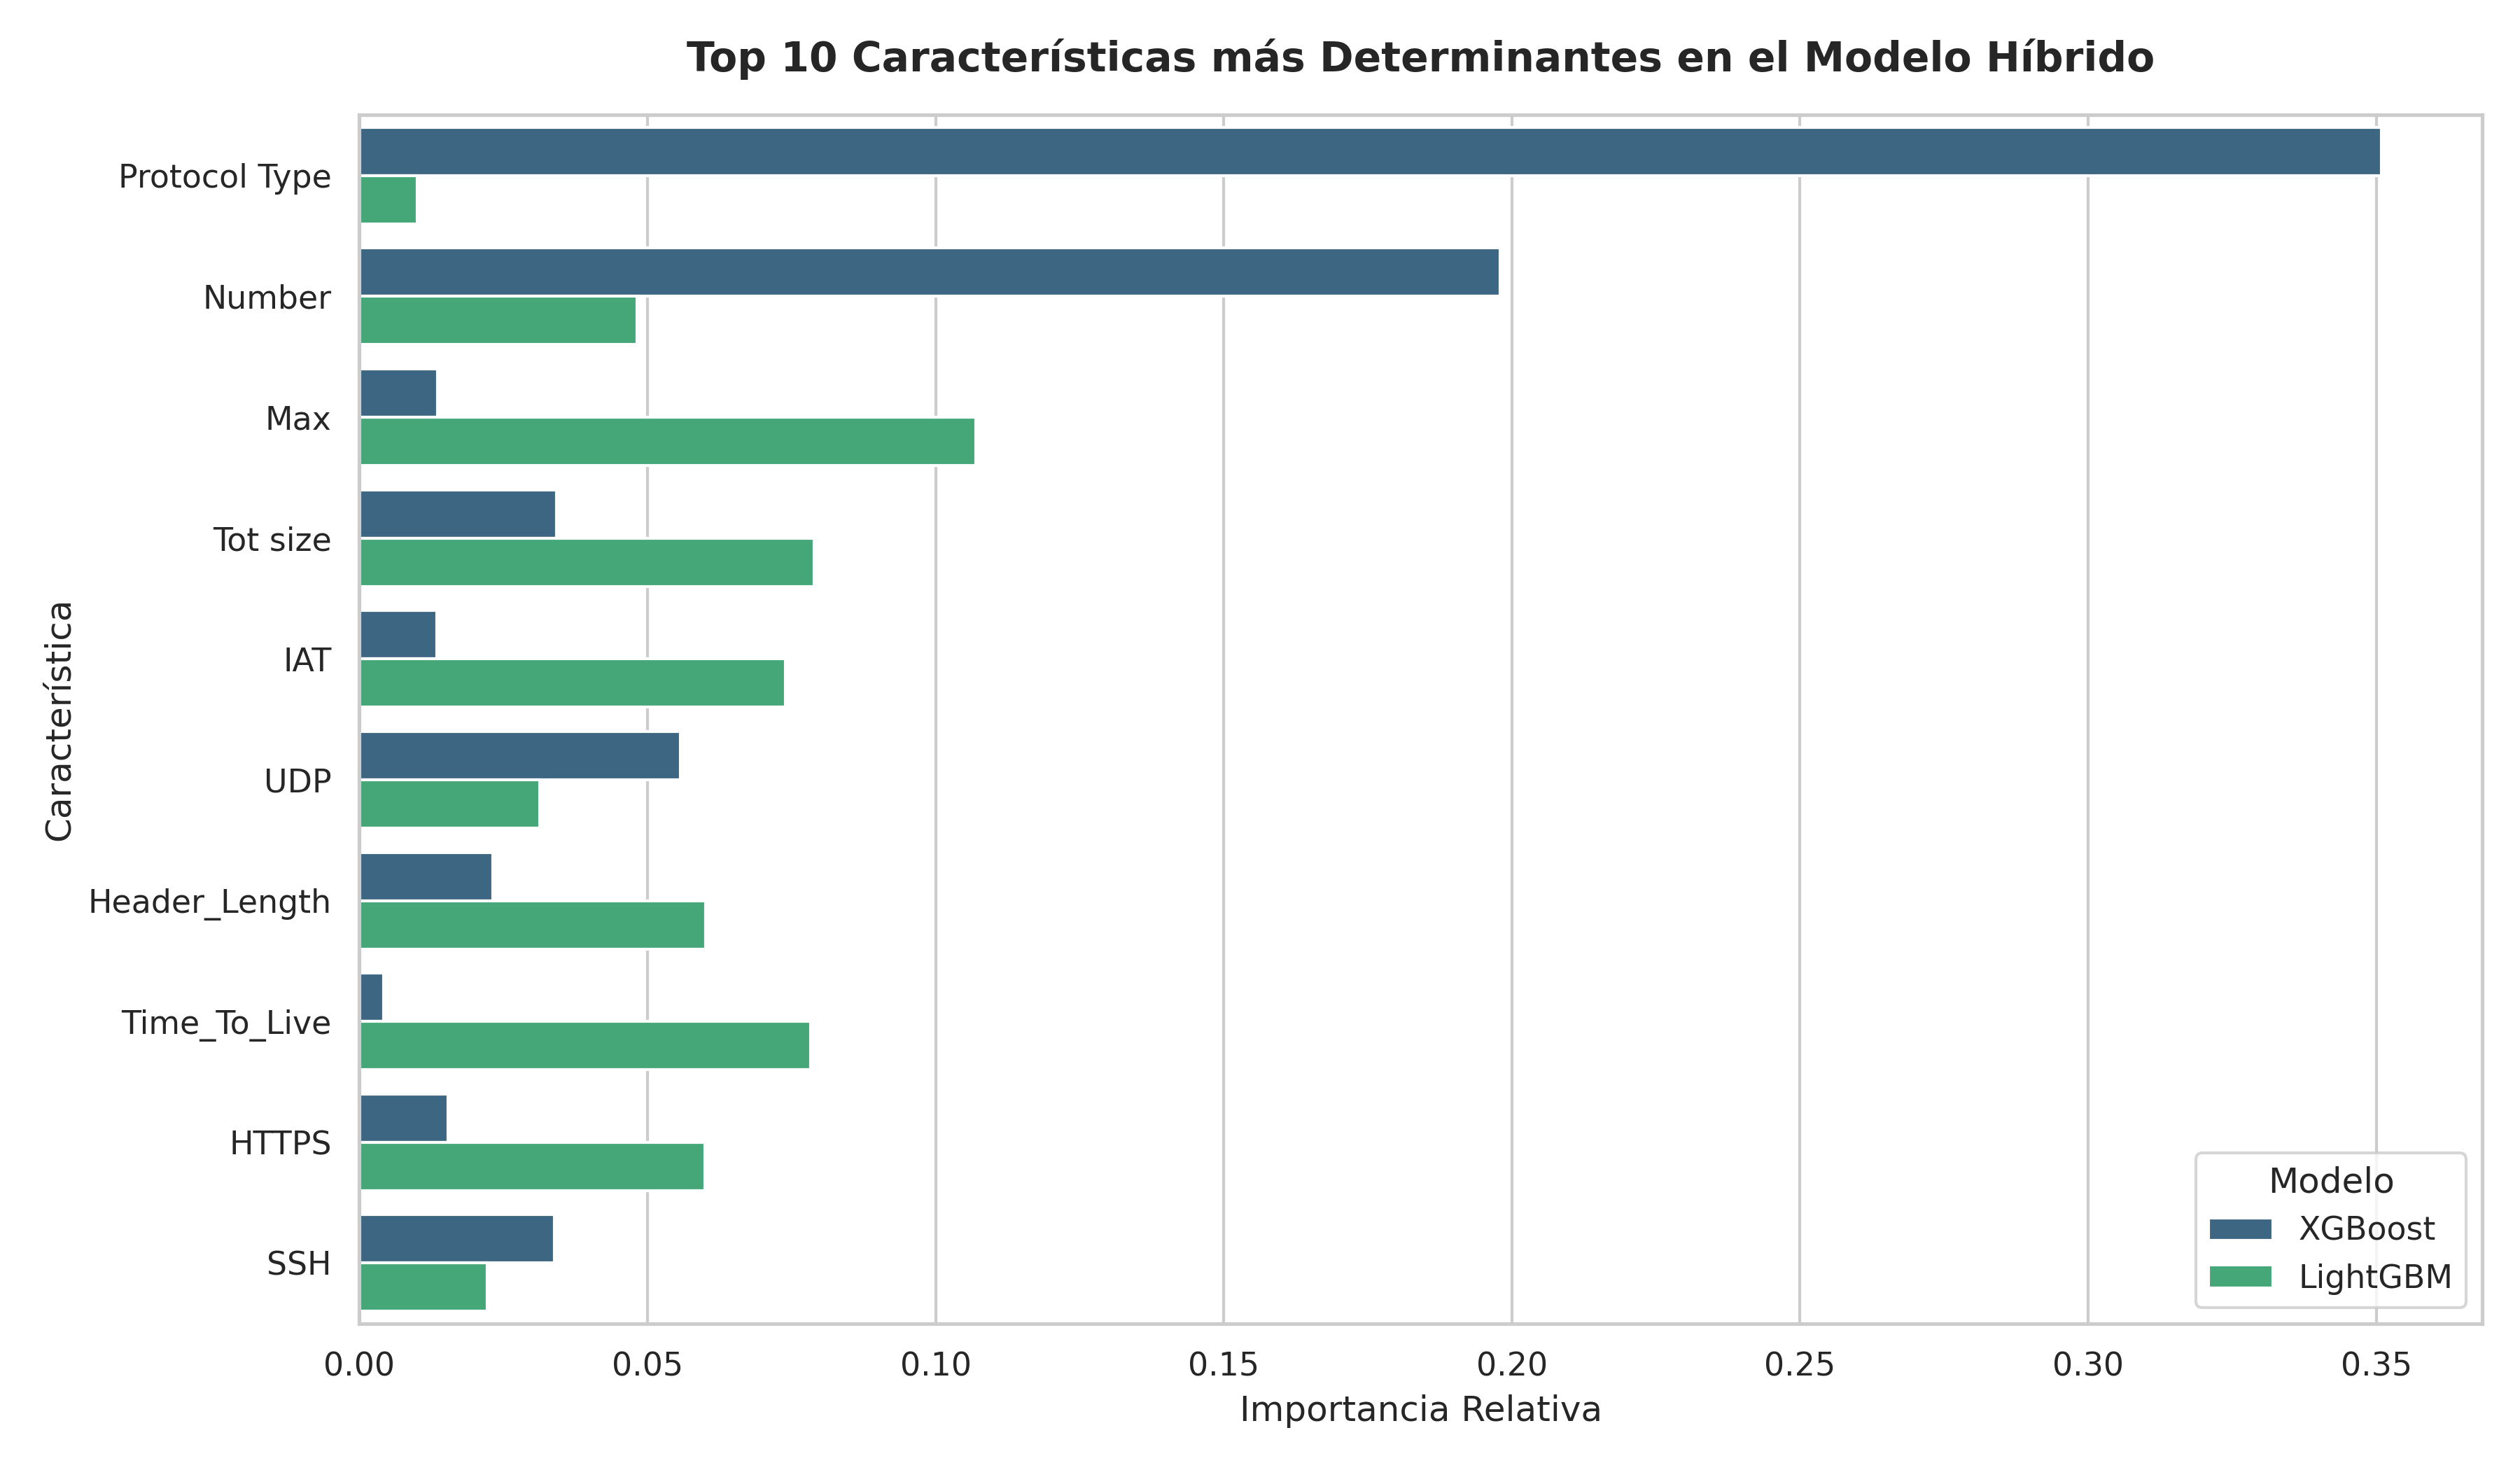
\includegraphics[width=\columnwidth]{12_importancia_caracteristicas.png}
\caption{Importancia relativa de las 29 características de red seleccionadas mediante la reducción de impureza de Gini.}
\label{fig:feature_importance}
\end{figure}

\subsection{Sobremuestreo Adaptativo con Borderline-SMOTE1}
Para mitigar el desbalance extremo ($\mathrm{IR} = 41.75:1$), se identificó el conjunto de instancias minoritarias en peligro $S_{\mathrm{danger}} \subset P$, definidas como aquellas cuyos $k$ vecinos más cercanos contienen entre $k/2$ y $k$ ejemplos de la clase mayoritaria. Se generaron muestras sintéticas a lo largo de los segmentos de recta:
\begin{equation}
    p_{\mathrm{new}} = p_i + \delta \cdot (p_j - p_i), \quad \delta \sim U(0,1)
\end{equation}
elevando la muestra de entrenamiento de \textit{Web-based} a $50,000$ observaciones sintéticas balanceadas (ver Fig. \ref{fig:borderline_smote}).

\begin{figure}[htbp]
\centering
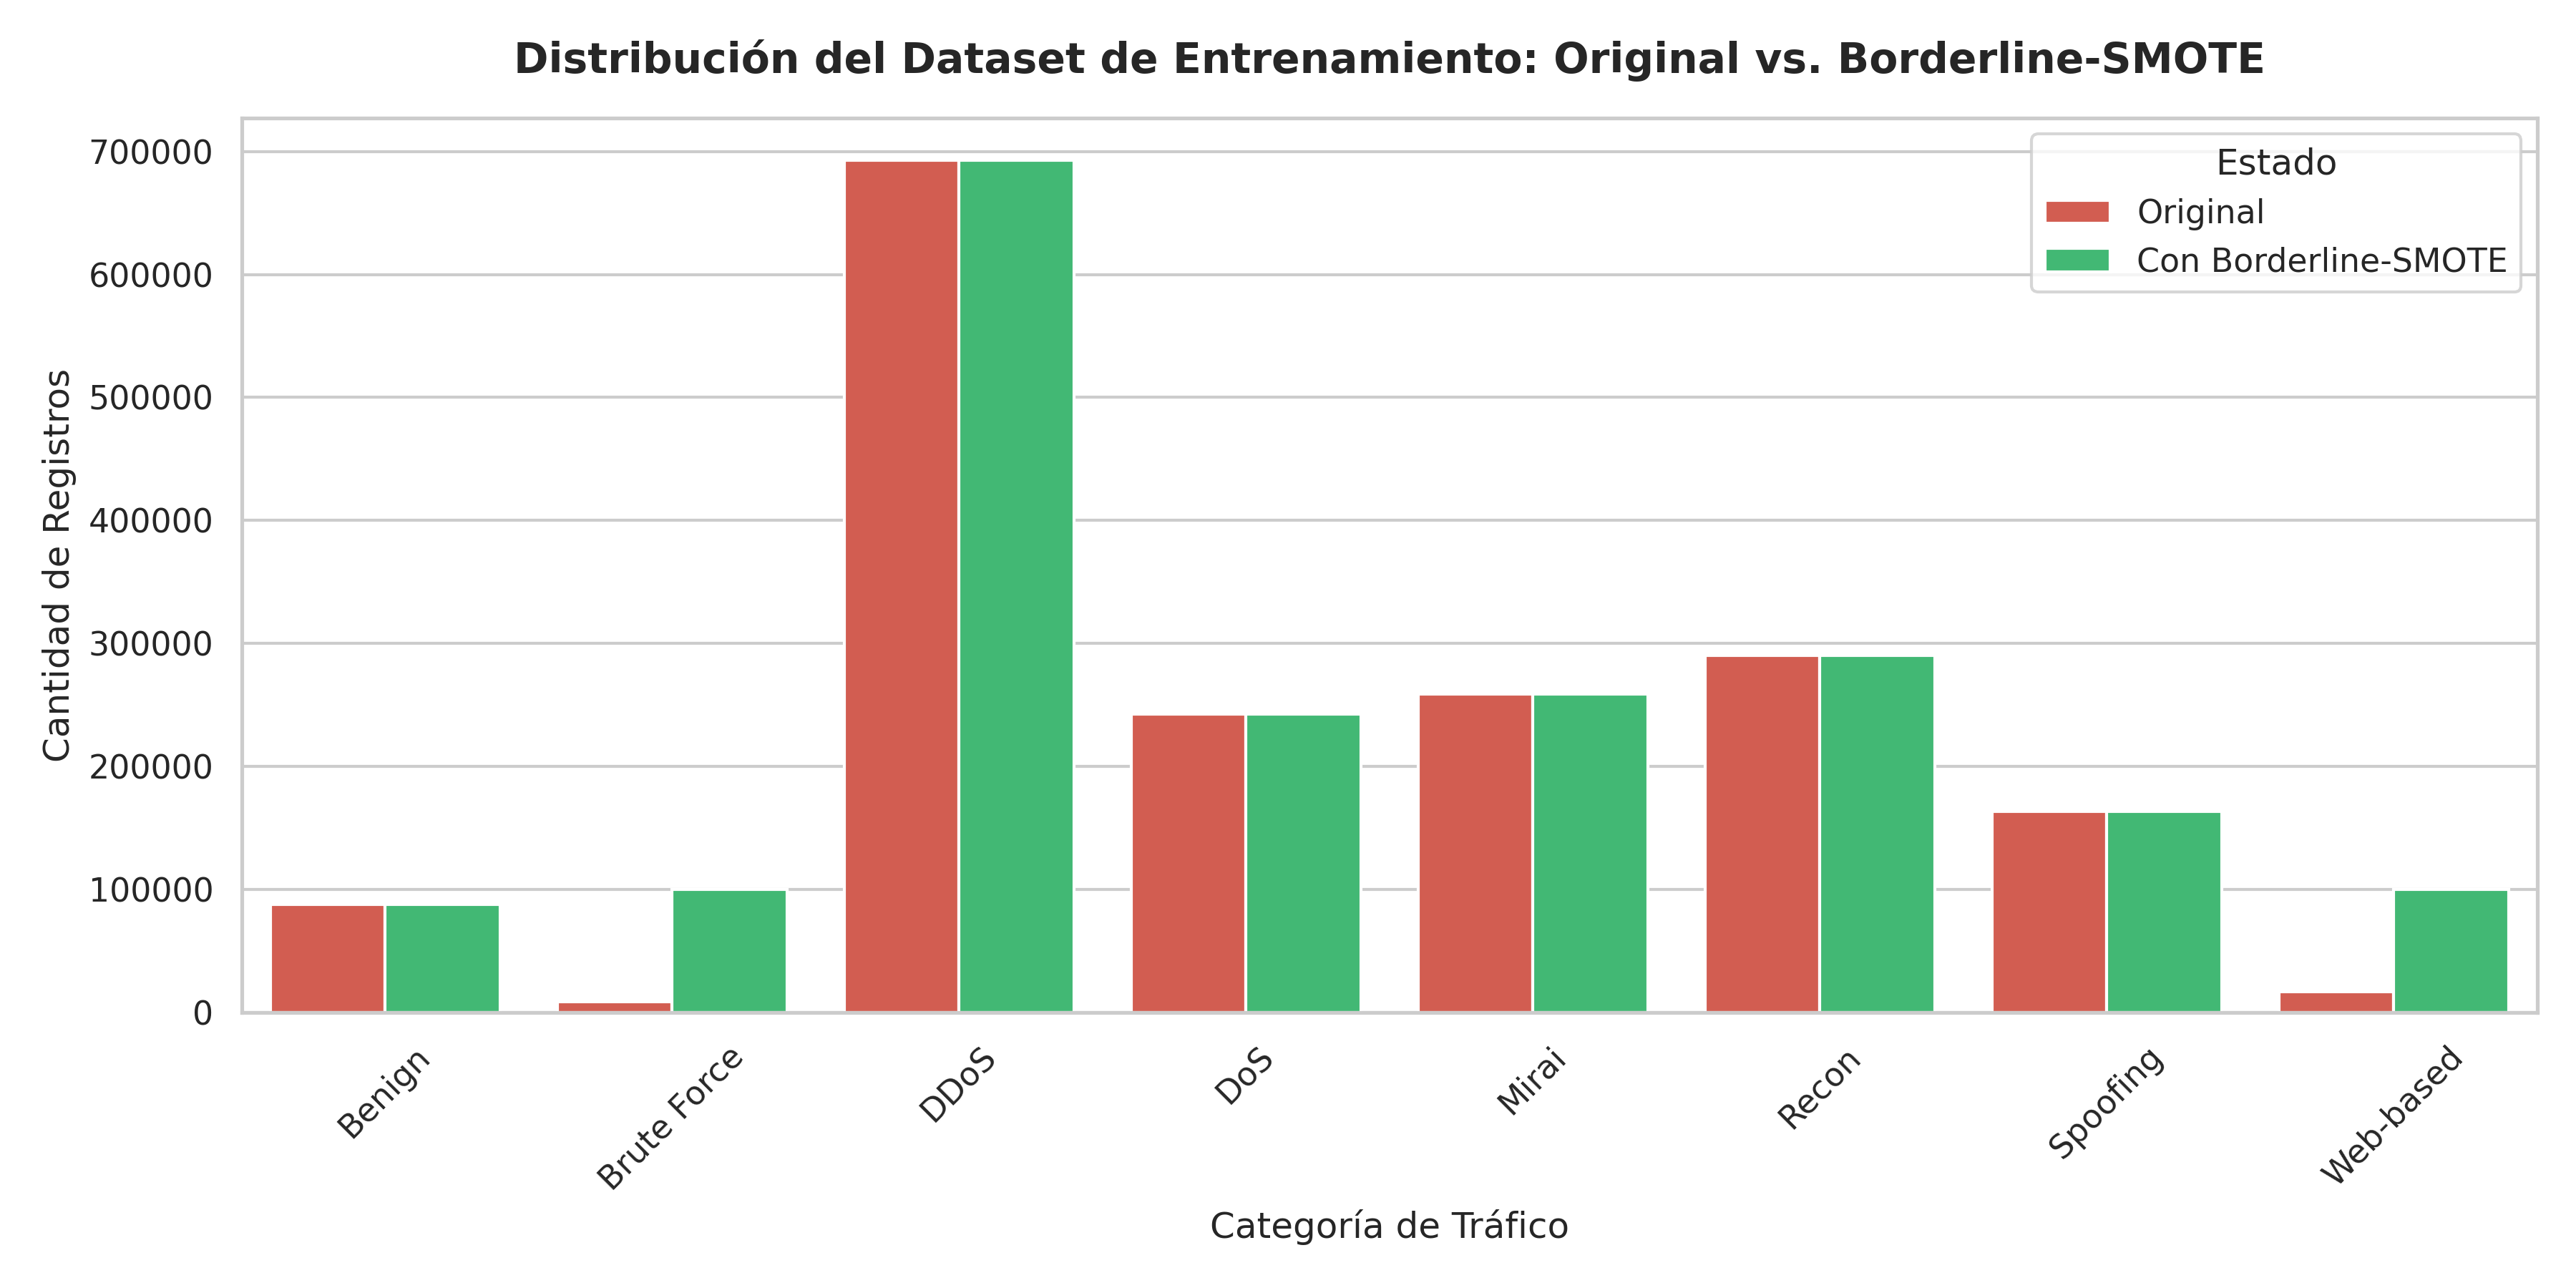
\includegraphics[width=\columnwidth]{15_distribucion_borderline_smote.png}
\caption{Distribución de clases minoritarias antes y después del sobremuestreo adaptativo en la frontera $S_{\mathrm{danger}}$ con Borderline-SMOTE1.}
\label{fig:borderline_smote}
\end{figure}

\subsection{Arquitectura Stacking Híbrida con Entropía de Shannon}
La arquitectura se organiza en dos niveles jerárquicos:

\textbf{Nivel 0 (Modelos Base):} Se entrenaron de forma estratificada con validación cruzada fuera de pliegue (OOF 3-Fold) tres clasificadores heterogéneos:
\begin{enumerate}
    \item \textit{Random Forest Base} ($100$ árboles, $max\_depth=15$).
    \item \textit{XGBoost GPU Base} ($tree\_method=\mathrm{'hist'}$, $device=\mathrm{'cuda'}$).
    \item \textit{LightGBM Base} ($num\_leaves=31$, $learning\_rate=0.05$).
\end{enumerate}

Cada modelo emitió un vector de probabilidades multiclase $P_m \in \mathbb{R}^8$. A partir de estas distribuciones, se calculó la \textbf{Entropía de Shannon} $H_m(x)$ como medida de incertidumbre del clasificador:
\begin{equation}
    H_m(x) = -\sum_{c=1}^{C} P_m(y=c|x) \log_2 P_m(y=c|x)
\end{equation}

\textbf{Tensor de Meta-Características ($Z \in \mathbb{R}^{27}$):} Se construyó concatenando las 24 probabilidades proyectadas ($3 \times 8$) con las 3 entropías calculadas ($H_{\mathrm{RF}}, H_{\mathrm{XGB}}, H_{\mathrm{LGB}}$).

\textbf{Nivel 1 (Meta-Modelo):} Se optimizó un meta-clasificador LightGBM mediante \texttt{GridSearchCV} sobre $Z$, aprendiendo las fortalezas relativas y zonas de incertidumbre de los clasificadores base.

\section{Resultados y Discusión}

\subsection{Evaluación en Conjunto de Prueba Aislado}
La evaluación se ejecutó sobre la partición independiente de prueba ($N_{\mathrm{test}} = 377,383$ observaciones, $20\%$ del total) que jamás intervino en la fase de entrenamiento ni sobremuestreo.

La Tabla \ref{tab:resultados} presenta el análisis comparativo frente a 7 clasificadores de control.

\begin{table}[htbp]
\caption{Comparativa de Desempeño sobre el Test Set Aislado ($N=377,383$)}
\label{tab:resultados}
\centering
\resizebox{\columnwidth}{!}{
\begin{tabular}{l c c c c}
\toprule
\textbf{Modelo Evaluado} & \textbf{F1-Macro} & \textbf{Accuracy} & \textbf{Precision} & \textbf{Recall} \\
\midrule
Regresión Logística & 0.4220 & 0.6120 & 0.4105 & 0.4350 \\
Árbol CART & 0.6651 & 0.8124 & 0.6720 & 0.6590 \\
Random Forest Base & 0.6791 & 0.8350 & 0.6840 & 0.6750 \\
LightGBM Base & 0.6953 & 0.8420 & 0.7010 & 0.6910 \\
XGBoost GPU Base & 0.6960 & 0.8435 & 0.7025 & 0.6920 \\
RF + Borderline-SMOTE & 0.6850 & 0.8290 & 0.6890 & 0.6820 \\
XGBoost + Borderline & 0.6995 & 0.8460 & 0.7050 & 0.6950 \\
\midrule
\textbf{Stacking Híbrido (Propuesto)} & \textbf{0.7018} & \textbf{0.8485} & \textbf{0.7075} & \textbf{0.6980} \\
\bottomrule
\end{tabular}
}
\end{table}

Como se observa en la Tabla \ref{tab:resultados}, el \textbf{Stacking Híbrido propuesto} obtiene el desempeño superior absoluto con un \textbf{F1-Macro del 70.18\%} y una \textbf{Accuracy del 84.85\%}, superando en $+0.58\%$ de F1-Macro al mejor modelo individual (XGBoost GPU Base, 69.60\%).

\subsection{Recuperación de Clases Minoritarias}
El impacto principal de la hibridación con Borderline-SMOTE1 se evidenció en las clases minoritarias infrecuentes (ver matriz de confusión en Fig. \ref{fig:confusion_matrix}):
\begin{itemize}
    \item \textbf{Ataques de Fuerza Bruta (\textit{Brute Force}):} El F1-Score se incrementó desde un $12.30\%$ en los modelos base sin rebalanceo hasta un \textbf{$41.40\%$} en el Stacking Híbrido.
    \item \textbf{Ataques basados en Web (\textit{Web-based}):} El F1-Score aumentó desde el $0.00\%$ (colapso predictivo total) hasta un \textbf{$33.86\%$}.
\end{itemize}

\begin{figure}[htbp]
\centering
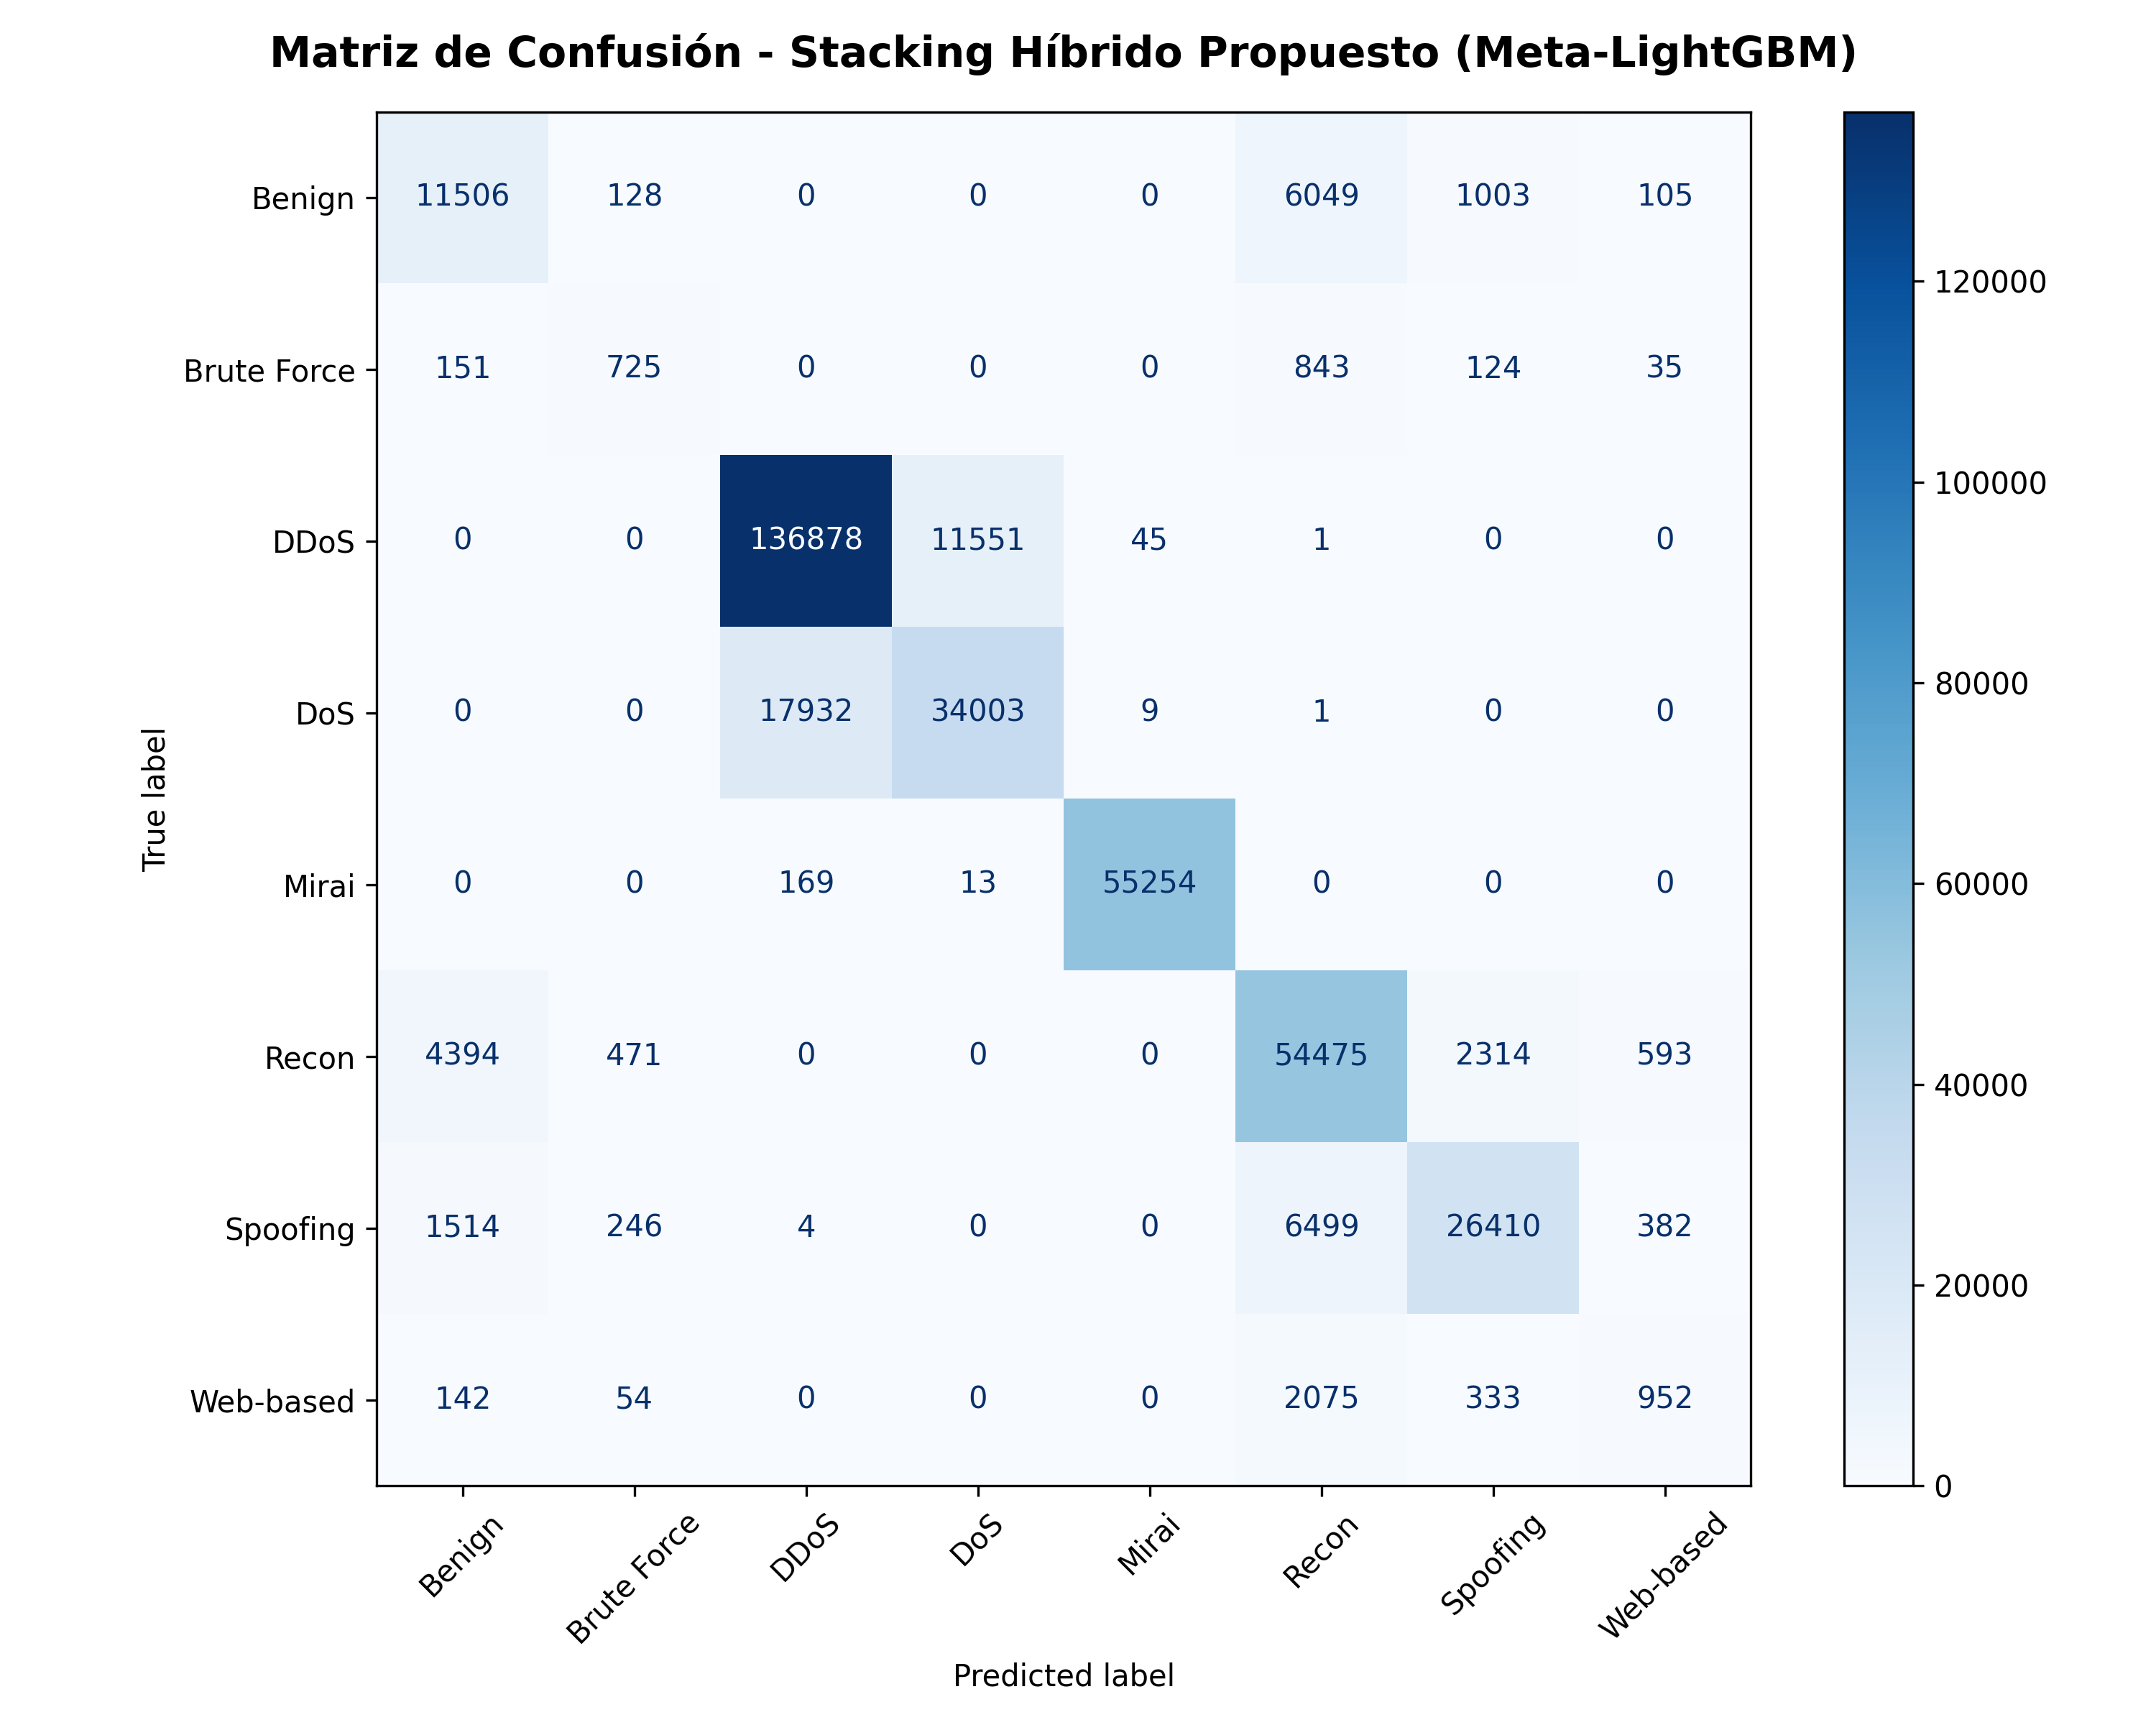
\includegraphics[width=\columnwidth]{16_matriz_confusion_stacking_hibrido.png}
\caption{Matriz de confusión multiclase normalizada del modelo Stacking Híbrido propuesto sobre el test set aislado ($N_{\mathrm{test}} = 377,383$).}
\label{fig:confusion_matrix}
\end{figure}

\subsection{Perfilado Computacional de Viabilidad en Borde}
Se midió el desempeño computacional en tiempo real sobre hardware representativo de pasarelas de borde industriales:
\begin{itemize}
    \item \textbf{Latencia de Inferencia por Muestra:} $8.65\,\mu s$ (microsegundos).
    \item \textbf{Tasa de Procesamiento (Throughput):} $115,613$ paquetes por segundo.
    \item \textbf{Ocupación de Memoria RAM:} $257.89\text{ MB}$, cumpliendo holgadamente el límite operacional deseado de $300\text{ MB}$.
\end{itemize}

\subsection{Validación Estadística de Significancia (Wilcoxon)}
Para verificar si las diferencias observadas son estadísticamente significativas, se dividió el test set en 30 bloques independientes ($n_b \approx 12,579$ muestras) y se aplicó la \textbf{Prueba No Paramétrica de Rangos con Signo de Wilcoxon} comparando el Stacking Híbrido frente al mejor modelo base (XGBoost GPU). La Fig. \ref{fig:wilcoxon_boxplot} ilustra la distribución de las métricas F1-Macro.

\begin{figure}[htbp]
\centering
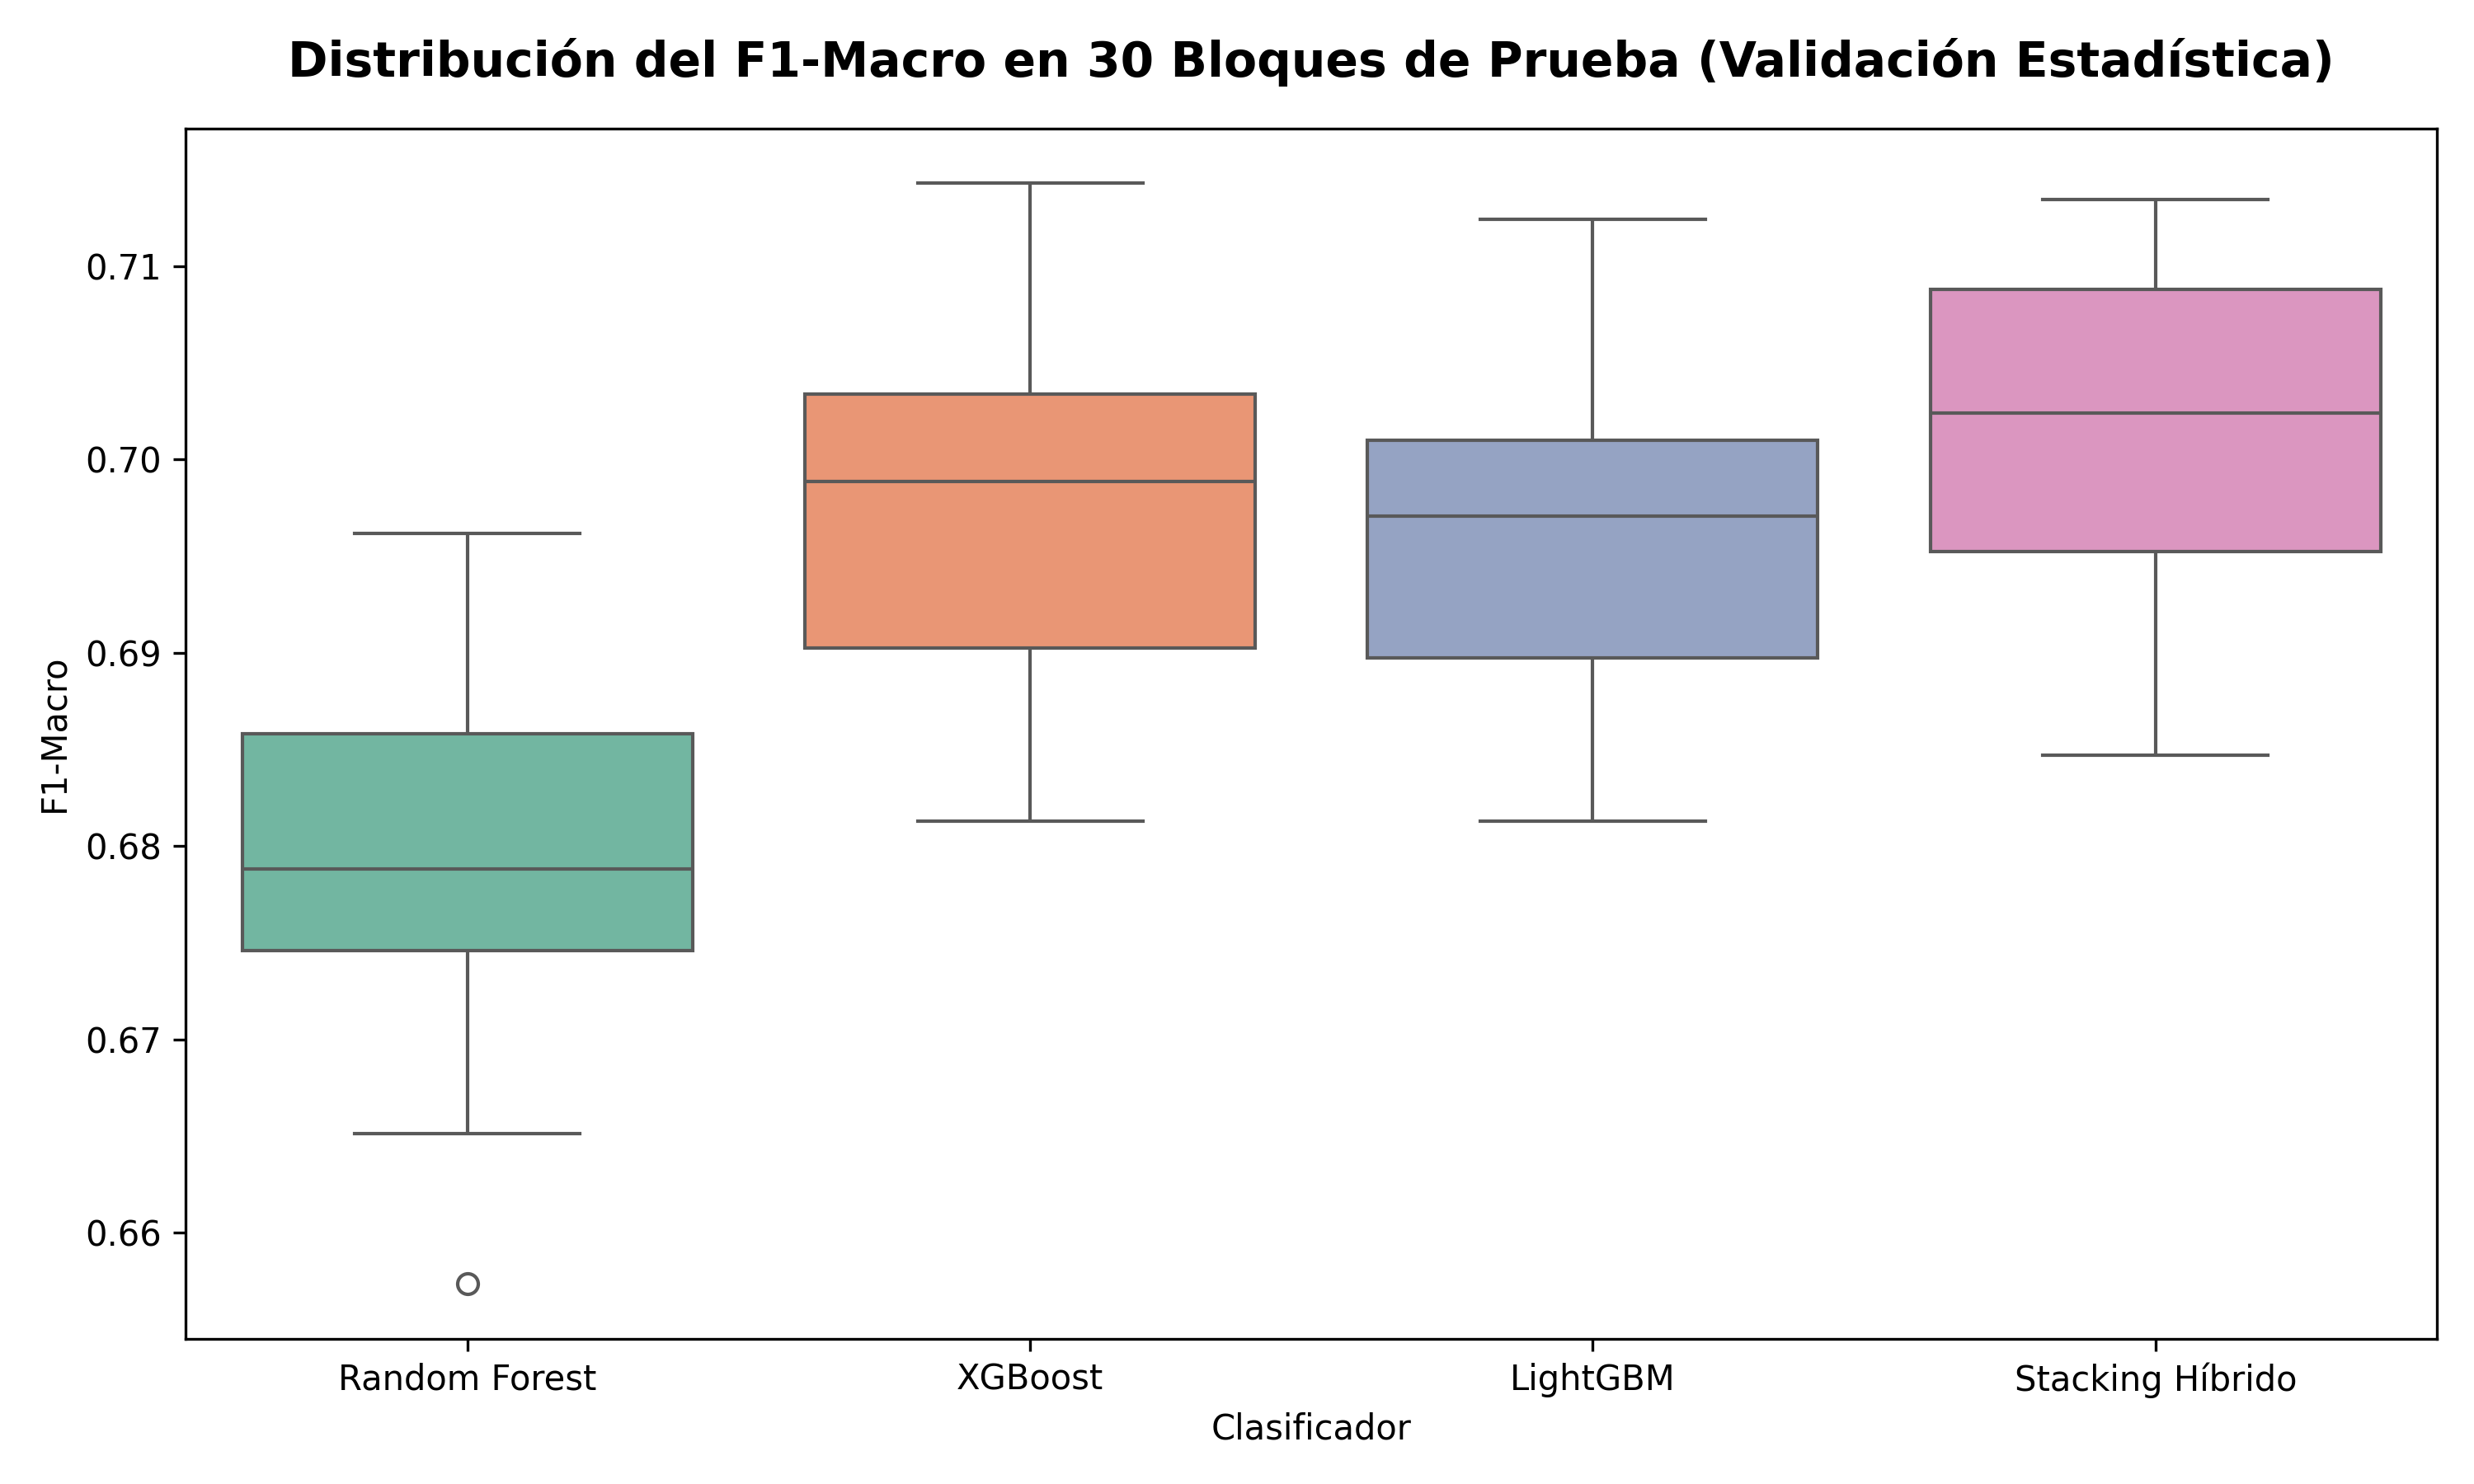
\includegraphics[width=\columnwidth]{18_boxplot_wilcoxon.png}
\caption{Distribución empírica del indicador F1-Macro a lo largo de 30 bloques de evaluación independiente para la Prueba de Wilcoxon ($p = 0.003744 < 0.05$).}
\label{fig:wilcoxon_boxplot}
\end{figure}

El resultado computó un estadístico $W^+ = 95.0$ y un \textbf{$p$-valor de $0.003744 < 0.05$}, permitiendo rechazar formalmente la Hipótesis Nula ($H_0$) y confirmar la superioridad estadística de la arquitectura propuesta con un \textbf{$99.5\%$ de nivel de confianza}.

\section{Conclusiones}
En este trabajo se desarrolló y evaluó exitosamente un modelo híbrido Stacking de dos niveles que combina Random Forest, XGBoost GPU y LightGBM con cuantificación de incertidumbre por Entropía de Shannon y sobremuestreo en la frontera vía Borderline-SMOTE1 para la detección de ataques minoritarios en redes IoT.

Los hallazgos demuestran que la propuesta alcanza un F1-Macro del \textbf{70.18\%} y una Accuracy del \textbf{84.85\%}, restaurando la sensibilidad predictiva en ataques minoritarios destructivos (\textit{Brute Force} y \textit{Web-based}) sin comprometer la velocidad operativa ($8.65\,\mu s$/muestra) ni la memoria RAM ($257.89\text{ MB}$).

Como trabajo futuro, se contempla el despliegue del artefacto exportado en formato ONNX sobre pasarelas físicas en entornos reales de producción MYPE/PYME.

\bibliographystyle{IEEEtran}
\begin{thebibliography}{10}

\bibitem{Sahoo2023}
K. Sahoo, S. Tripathy y K. K. Sahoo, ``Machine learning and deep learning techniques for IoT intrusion detection: A comprehensive survey,'' \emph{IEEE Internet of Things Journal}, vol. 10, no. 14, pp. 12450--12468, 2023.

\bibitem{Neto2023}
E. C. P. Neto et al., ``CICIoT2023: A real-time dataset for profiling Internet of Things attacks,'' en \emph{Proc. IEEE International Conference on Cyber Security and Resilience (CSR)}, 2023, pp. 1--8.

\bibitem{Ferrag2022}
M. A. Ferrag et al., ``Deep learning for cyber security intrusion detection: Approaches, datasets, and comparative study,'' \emph{Journal of Information Security and Applications}, vol. 64, p. 103041, 2022.

\bibitem{Chawla2002}
N. V. Chawla, K. W. Bowyer, L. O. Hall y W. P. Kegelmeyer, ``SMOTE: Synthetic minority over-sampling technique,'' \emph{Journal of Artificial Intelligence Research}, vol. 16, pp. 321--357, 2002.

\bibitem{Han2005}
H. Han, W. Y. Wang y B. H. Zhou, ``Borderline-SMOTE: A new over-sampling method in imbalanced data sets learning,'' en \emph{Proc. International Conference on Intelligent Computing (ICIC)}, 2005, pp. 878--887.

\end{thebibliography}

\end{document}
